\documentclass[slides]{beamer} %switch "slides" to "handout" for printing out
%\documentclass[handout]{beamer}

%packages
%\usepackage{latexsym}
\usepackage{graphicx}
\usepackage{color}
\usepackage{amsmath}
\usepackage{dsfont}
%\usepackage{placeins}
\usepackage{amssymb}
%\usepackage{wasysym}
%\usepackage{abstract}
\usepackage{hyperref}
\usepackage{cancel}
%\usepackage[margin=1.05in]{geometry}
%\usepackage{enumerate}
\usepackage{listings}
\usepackage{mathdots}
\usepackage{cancel}
\usepackage{array}
\usepackage{algorithm}
\usepackage{algorithmic}
\usepackage{multirow}

\usepackage{tikz}
\usepackage{amsmath}
\usepackage{verbatim}
\usetikzlibrary{arrows,shapes}

\newcommand{\tikzmark}[1]{\tikz[remember picture] \node[coordinate] (#1) {#1};}

\lstset{language = R, numbers = left, backgroundcolor = \color{backgcode}, title = \lstname, breaklines = true, basicstyle = \small, commentstyle = \footnotesize\color{Brown}, stringstyle = \ttfamily, tabsize = 2, fontadjust = true, showspaces = false, showstringspaces = false, texcl = true, numbers = none}

\newcounter{probnum}
\setcounter{probnum}{1}

%create definition to allow local margin changes
\def\changemargin#1#2{\list{}{\rightmargin#2\leftmargin#1}\item[]}
\let\endchangemargin=\endlist 

%allow equations to span multiple pages
\allowdisplaybreaks

%define colors and color typesetting conveniences
\definecolor{gray}{rgb}{0.7,0.7,0.7}
\newcommand{\ingray}[1]{\color{gray}#1 \color{black}}
\definecolor{black}{rgb}{0,0,0}
\definecolor{white}{rgb}{1,1,1}
\definecolor{blue}{rgb}{0,0,0.7}
\newcommand{\inblue}[1]{\color{blue}#1 \color{black}}
\definecolor{green}{rgb}{0.133,0.545,0.133}
\newcommand{\ingreen}[1]{\color{green}#1 \color{black}}
\definecolor{yellow}{rgb}{1,0.549,0}
\newcommand{\inyellow}[1]{\color{yellow}#1 \color{black}}
\definecolor{red}{rgb}{1,0.133,0.133}
\newcommand{\inred}[1]{\color{red}#1 \color{black}}
\definecolor{purple}{rgb}{0.58,0,0.827}
\newcommand{\inpurple}[1]{\color{purple}#1 \color{black}}
\definecolor{backgcode}{rgb}{0.97,0.97,0.8}
\definecolor{Brown}{cmyk}{0,0.81,1,0.60}
\definecolor{OliveGreen}{cmyk}{0.64,0,0.95,0.40}
\definecolor{CadetBlue}{cmyk}{0.62,0.57,0.23,0}

%define new math operators
\DeclareMathOperator*{\argmax}{arg\,max~}
\DeclareMathOperator*{\argmin}{arg\,min~}
\DeclareMathOperator*{\argsup}{arg\,sup~}
\DeclareMathOperator*{\arginf}{arg\,inf~}
\DeclareMathOperator*{\convolution}{\text{\Huge{$\ast$}}}
\newcommand{\infconv}[2]{\convolution^\infty_{#1 = 1} #2}
%true functions

%%%% GENERAL SHORTCUTS

%shortcuts for pure typesetting conveniences
\newcommand{\bv}[1]{\boldsymbol{#1}}

%shortcuts for compound constants
\newcommand{\BetaDistrConst}{\dfrac{\Gamma(\alpha + \beta)}{\Gamma(\alpha)\Gamma(\beta)}}
\newcommand{\NormDistrConst}{\dfrac{1}{\sqrt{2\pi\sigma^2}}}

\newcommand{\qu}[1]{``#1''}
%shortcuts for conventional symbols
\newcommand{\tsq}{\tau^2}
\newcommand{\tsqh}{\hat{\tau}^2}
\newcommand{\sigsq}{\sigma^2}
\newcommand{\sigsqsq}{\parens{\sigma^2}^2}
\newcommand{\sigsqovern}{\dfrac{\sigsq}{n}}
\newcommand{\tausq}{\tau^2}
\newcommand{\tausqalpha}{\tau^2_\alpha}
\newcommand{\tausqbeta}{\tau^2_\beta}
\newcommand{\tausqsigma}{\tau^2_\sigma}
\newcommand{\betasq}{\beta^2}
\newcommand{\sigsqvec}{\bv{\sigma}^2}
\newcommand{\sigsqhat}{\hat{\sigma}^2}
\newcommand{\Omegahat}{\hat{\Omega}}
\newcommand{\sigsqhatmlebayes}{\sigsqhat_{\text{Bayes, MLE}}}
\newcommand{\sigsqhatmle}[1]{\sigsqhat_{#1, \text{MLE}}}
\newcommand{\bSigma}{\bv{\Sigma}}
\newcommand{\bSigmainv}{\bSigma^{-1}}
\newcommand{\gammavec}{\bv{\gamma}}
\newcommand{\thetavec}{\bv{\theta}}
\newcommand{\thetahat}{\hat{\theta}}
\newcommand{\thetavechat}{\hat{\thetavec}}
\newcommand{\thetahatmle}{\hat{\theta}_{\mathrm{MLE}}}
\newcommand{\thetavechatmle}{\hat{\thetavec}_{\mathrm{MLE}}}
\newcommand{\pihatmle}{\hat{\pi}_{\mathrm{MLE}}}
\newcommand{\muhat}{\hat{\mu}}
\newcommand{\musq}{\mu^2}
\newcommand{\muvec}{\bv{\mu}}
\newcommand{\pivec}{\bv{\pi}}
\newcommand{\muhatmle}{\muhat_{\text{MLE}}}
\newcommand{\lambdahat}{\hat{\lambda}}
\newcommand{\lambdahatmle}{\lambdahat_{\text{MLE}}}
\newcommand{\lambdahatmleone}{\lambdahat_{\text{MLE}, 1}}
\newcommand{\lambdahatmletwo}{\lambdahat_{\text{MLE}, 2}}
\newcommand{\etavec}{\bv{\eta}}
\newcommand{\alphavec}{\bv{\alpha}}
\newcommand{\minimaxdec}{\delta^*_{\mathrm{mm}}}
\newcommand{\ybar}{\bar{y}}
\newcommand{\Ybar}{\bar{Y}}
\newcommand{\xbar}{\bar{x}}
\newcommand{\Xbar}{\bar{X}}
\newcommand{\zbar}{\bar{z}}
\newcommand{\Zbar}{\bar{Z}}

\newcommand{\seteq}{~{\buildrel set \over =}~}
\newcommand{\iid}{~{\buildrel iid \over \sim}~}
\newcommand{\inddist}{~{\buildrel ind \over \sim}~}
\newcommand{\approxdist}{~~{\buildrel approx \over \sim}~~}
\newcommand{\equalsindist}{~{\buildrel d \over =}~}
\newcommand{\equalsquestion}{~{\buildrel ? \over =}~}
\newcommand{\geqquestion}{~{\buildrel ? \over \geq}~}
\newcommand{\lik}[1]{L\parens{#1}}
\newcommand{\loglik}[1]{\ell\parens{#1}}
\newcommand{\thetahatkminone}{\thetahat^{(k-1)}}
\newcommand{\thetahatkplusone}{\thetahat^{(k+1)}}
\newcommand{\thetahatk}{\thetahat^{(k)}}
\newcommand{\half}{\frac{1}{2}}
\newcommand{\third}{\frac{1}{3}}
\newcommand{\twothirds}{\frac{2}{3}}
\newcommand{\fourth}{\frac{1}{4}}
\newcommand{\fifth}{\frac{1}{5}}
\newcommand{\sixth}{\frac{1}{6}}

%shortcuts for vector and matrix notation
\newcommand{\A}{\bv{A}}
\newcommand{\At}{\A^T}
\newcommand{\Ainv}{\inverse{\A}}
\newcommand{\B}{\bv{B}}
\newcommand{\C}{\bv{C}}
\newcommand{\K}{\bv{K}}
\newcommand{\Kt}{\K^T}
\newcommand{\Kinv}{\inverse{K}}
\newcommand{\Kinvt}{(\Kinv)^T}
\newcommand{\M}{\bv{M}}
\newcommand{\Bt}{\B^T}
\newcommand{\Q}{\bv{Q}}
\newcommand{\E}{\bv{E}}
\newcommand{\Et}{\E^\top}
\newcommand{\Qt}{\Q^T}
\newcommand{\R}{\bv{R}}
\newcommand{\Rt}{\R^\top}
\newcommand{\Z}{\bv{Z}}
\newcommand{\X}{\bv{X}}
\renewcommand{\H}{\bv{H}}
\newcommand{\Xsub}{\X_{\text{(sub)}}}
\newcommand{\Xsubadj}{\X_{\text{(sub,adj)}}}
\newcommand{\I}{\bv{I}}
\newcommand{\J}{\bv{J}}
\newcommand{\0}{\bv{0}}
\newcommand{\1}{\bv{1}}
\newcommand{\Y}{\bv{Y}}
\newcommand{\Yt}{\Y^\top}
\newcommand{\tvec}{\bv{t}}
\newcommand{\sigsqI}{\sigsq\I}
\renewcommand{\P}{\bv{P}}
\newcommand{\Psub}{\P_{\text{(sub)}}}
\newcommand{\Pt}{\P^T}
\newcommand{\Pii}{P_{ii}}
\newcommand{\Pij}{P_{ij}}
\newcommand{\IminP}{(\I-\P)}
\newcommand{\Xt}{\bv{X}^T}
\newcommand{\XtX}{\Xt\X}
\newcommand{\XtXinv}{\parens{\Xt\X}^{-1}}
\newcommand{\XtXinvXt}{\XtXinv\Xt}
\newcommand{\XXtXinvXt}{\X\XtXinvXt}
\newcommand{\x}{\bv{x}}
\newcommand{\onevec}{\bv{1}}
\newcommand{\zerovec}{\bv{0}}
\newcommand{\onevectr}{\onevec^\top}
\newcommand{\oneton}{1, \ldots, n}
\newcommand{\yoneton}{y_1, \ldots, y_n}
\newcommand{\yonetonorder}{y_{(1)}, \ldots, y_{(n)}}
\newcommand{\Yoneton}{Y_1, \ldots, Y_n}
\newcommand{\iinoneton}{i \in \braces{\oneton}}
\newcommand{\onetom}{1, \ldots, m}
\newcommand{\jinonetom}{j \in \braces{\onetom}}
\newcommand{\xoneton}{x_1, \ldots, x_n}
\newcommand{\Xoneton}{X_1, \ldots, X_n}
\newcommand{\xt}{\x^T}
\newcommand{\y}{\bv{y}}
\newcommand{\yt}{\y^T}
\newcommand{\n}{\bv{n}}
\renewcommand{\c}{\bv{c}}
\newcommand{\ct}{\c^T}
\newcommand{\tstar}{\bv{t}^*}
\renewcommand{\u}{\bv{u}}
\renewcommand{\v}{\bv{v}}
\renewcommand{\a}{\bv{a}}
\newcommand{\s}{\bv{s}}
\newcommand{\yadj}{\y_{\text{(adj)}}}
\newcommand{\xjadj}{\x_{j\text{(adj)}}}
\newcommand{\xjadjM}{\x_{j \perp M}}
\newcommand{\yhat}{\hat{\y}}
\newcommand{\yhatsub}{\yhat_{\text{(sub)}}}
\newcommand{\yhatstar}{\yhat^*}
\newcommand{\yhatstarnew}{\yhatstar_{\text{new}}}
\newcommand{\z}{\bv{z}}
\newcommand{\zt}{\z^T}
\newcommand{\bb}{\bv{b}}
\newcommand{\bbt}{\bb^T}
\newcommand{\bbeta}{\bv{\beta}}
\newcommand{\beps}{\bv{\epsilon}}
\newcommand{\bepst}{\beps^T}
\newcommand{\e}{\bv{e}}
\newcommand{\Mofy}{\M(\y)}
\newcommand{\KofAlpha}{K(\alpha)}
\newcommand{\ellset}{\mathcal{L}}
\newcommand{\oneminalph}{1-\alpha}
\newcommand{\SSE}{\text{SSE}}
\newcommand{\SSEsub}{\text{SSE}_{\text{(sub)}}}
\newcommand{\MSE}{\text{MSE}}
\newcommand{\RMSE}{\text{RMSE}}
\newcommand{\SSR}{\text{SSR}}
\newcommand{\SST}{\text{SST}}
\newcommand{\JSest}{\delta_{\text{JS}}(\x)}
\newcommand{\Bayesest}{\delta_{\text{Bayes}}(\x)}
\newcommand{\EmpBayesest}{\delta_{\text{EmpBayes}}(\x)}
\newcommand{\BLUPest}{\delta_{\text{BLUP}}}
\newcommand{\MLEest}[1]{\hat{#1}_{\text{MLE}}}

%shortcuts for Linear Algebra stuff (i.e. vectors and matrices)
\newcommand{\twovec}[2]{\bracks{\begin{array}{c} #1 \\ #2 \end{array}}}
\newcommand{\threevec}[3]{\bracks{\begin{array}{c} #1 \\ #2 \\ #3 \end{array}}}
\newcommand{\fivevec}[5]{\bracks{\begin{array}{c} #1 \\ #2 \\ #3 \\ #4 \\ #5 \end{array}}}
\newcommand{\twobytwomat}[4]{\bracks{\begin{array}{cc} #1 & #2 \\ #3 & #4 \end{array}}}
\newcommand{\threebytwomat}[6]{\bracks{\begin{array}{cc} #1 & #2 \\ #3 & #4 \\ #5 & #6 \end{array}}}

%shortcuts for conventional compound symbols
\newcommand{\thetainthetas}{\theta \in \Theta}
\newcommand{\reals}{\mathbb{R}}
\newcommand{\complexes}{\mathbb{C}}
\newcommand{\rationals}{\mathbb{Q}}
\newcommand{\integers}{\mathbb{Z}}
\newcommand{\naturals}{\mathbb{N}}
\newcommand{\forallninN}{~~\forall n \in \naturals}
\newcommand{\forallxinN}[1]{~~\forall #1 \in \reals}
\newcommand{\matrixdims}[2]{\in \reals^{\,#1 \times #2}}
\newcommand{\inRn}[1]{\in \reals^{\,#1}}
\newcommand{\mathimplies}{\quad\Rightarrow\quad}
\newcommand{\mathequiv}{\quad\Leftrightarrow\quad}
\newcommand{\eqncomment}[1]{\quad \text{(#1)}}
\newcommand{\limitn}{\lim_{n \rightarrow \infty}}
\newcommand{\limitN}{\lim_{N \rightarrow \infty}}
\newcommand{\limitd}{\lim_{d \rightarrow \infty}}
\newcommand{\limitt}{\lim_{t \rightarrow \infty}}
\newcommand{\limitsupn}{\limsup_{n \rightarrow \infty}~}
\newcommand{\limitinfn}{\liminf_{n \rightarrow \infty}~}
\newcommand{\limitk}{\lim_{k \rightarrow \infty}}
\newcommand{\limsupn}{\limsup_{n \rightarrow \infty}}
\newcommand{\limsupk}{\limsup_{k \rightarrow \infty}}
\newcommand{\floor}[1]{\left\lfloor #1 \right\rfloor}
\newcommand{\ceil}[1]{\left\lceil #1 \right\rceil}

%shortcuts for environments
\newcommand{\beqn}{\vspace{-0.25cm}\begin{eqnarray*}}
\newcommand{\eeqn}{\end{eqnarray*}}
\newcommand{\bneqn}{\vspace{-0.25cm}\begin{eqnarray}}
\newcommand{\eneqn}{\end{eqnarray}}

\newcommand{\beans}{\color{blue} \beqn  \text{Ans:}~~~}
\newcommand{\eeans}{\eeqn \color{black}}

%shortcuts for mini environments
\newcommand{\parens}[1]{\left(#1\right)}
\newcommand{\squared}[1]{\parens{#1}^2}
\newcommand{\angbraces}[1]{\left<#1\right>}
\newcommand{\tothepow}[2]{\parens{#1}^{#2}}
\newcommand{\prob}[1]{\mathbb{P}\parens{#1}}
\newcommand{\supp}[1]{\mathbb{S}\text{upp}\bracks{#1}}
\newcommand{\cprob}[2]{\prob{#1~|~#2}}
\newcommand{\littleo}[1]{o\parens{#1}}
\newcommand{\bigo}[1]{O\parens{#1}}
\newcommand{\Lp}[1]{\mathbb{L}^{#1}}
\renewcommand{\arcsin}[1]{\text{arcsin}\parens{#1}}
\newcommand{\prodonen}[2]{\prod_{#1=1}^n #2}
\newcommand{\mysum}[4]{\sum_{#1=#2}^{#3} #4}
\newcommand{\sumonen}[2]{\sum_{#1=1}^n #2}
\newcommand{\infsum}[2]{\sum_{#1=1}^\infty #2}
\newcommand{\infprod}[2]{\prod_{#1=1}^\infty #2}
\newcommand{\infunion}[2]{\bigcup_{#1=1}^\infty #2}
\newcommand{\infinter}[2]{\bigcap_{#1=1}^\infty #2}
\newcommand{\infintegral}[2]{\int^\infty_{-\infty} #2 ~\text{d}#1}
\newcommand{\supthetas}[1]{\sup_{\thetainthetas}\braces{#1}}
\newcommand{\bracks}[1]{\left[#1\right]}
\newcommand{\braces}[1]{\left\{#1\right\}}
\newcommand{\set}[1]{\left\{#1\right\}}
\newcommand{\abss}[1]{\left|#1\right|}
\newcommand{\norm}[1]{\left|\left|#1\right|\right|}
\newcommand{\normsq}[1]{\norm{#1}^2}
\newcommand{\inverse}[1]{\parens{#1}^{-1}}
\newcommand{\rowof}[2]{\parens{#1}_{#2\cdot}}

%shortcuts for functionals
\newcommand{\realcomp}[1]{\text{Re}\bracks{#1}}
\newcommand{\imagcomp}[1]{\text{Im}\bracks{#1}}
\newcommand{\range}[1]{\text{range}\bracks{#1}}
\newcommand{\colsp}[1]{\text{colsp}\bracks{#1}}
\newcommand{\rowsp}[1]{\text{rowsp}\bracks{#1}}
\newcommand{\tr}[1]{\text{tr}\bracks{#1}}
\newcommand{\diag}[1]{\text{diag}\bracks{#1}}
\newcommand{\rank}[1]{\text{rank}\bracks{#1}}
\newcommand{\proj}[2]{\text{Proj}_{#1}\bracks{#2}}
\newcommand{\projcolspX}[1]{\text{Proj}_{\colsp{\X}}\bracks{#1}}
\newcommand{\median}[1]{\text{median}\bracks{#1}}
\newcommand{\mean}[1]{\text{mean}\bracks{#1}}
\newcommand{\dime}[1]{\text{dim}\bracks{#1}}
\renewcommand{\det}[1]{\text{det}\bracks{#1}}
\newcommand{\expe}[1]{\mathbb{E}\bracks{#1}}
\newcommand{\cexpe}[2]{\expe{#1 ~ | ~ #2}}
\newcommand{\expeabs}[1]{\expe{\abss{#1}}}
\newcommand{\expesub}[2]{\mathbb{E}_{#1}\bracks{#2}}
\newcommand{\indic}[1]{\mathds{1}_{#1}}
\newcommand{\var}[1]{\mathbb{V}\text{ar}\bracks{#1}}
\newcommand{\cvar}[2]{\var{#1~|~#2}}
\newcommand{\varhat}[1]{\hat{\mathbb{V}\text{ar}}\bracks{#1}}
\newcommand{\cov}[2]{\mathbb{C}\text{ov}\bracks{#1, #2}}
\newcommand{\corr}[2]{\text{Corr}\bracks{#1, #2}}
\newcommand{\se}[1]{\text{SE}\bracks{#1}}
\newcommand{\seest}[1]{\hat{\text{SE}}\bracks{#1}}
\newcommand{\bias}[1]{\text{Bias}\bracks{#1}}
\newcommand{\partialop}[2]{\dfrac{\partial}{\partial #1}\bracks{#2}}
\newcommand{\secpartialop}[2]{\dfrac{\partial^2}{\partial #1^2}\bracks{#2}}
\newcommand{\mixpartialop}[3]{\dfrac{\partial^2}{\partial #1 \partial #2}\bracks{#3}}

%shortcuts for functions
\renewcommand{\exp}[1]{\mathrm{exp}\parens{#1}}
\renewcommand{\cos}[1]{\text{cos}\parens{#1}}
\renewcommand{\sin}[1]{\text{sin}\parens{#1}}
\newcommand{\sign}[1]{\text{sign}\parens{#1}}
\newcommand{\are}[1]{\mathrm{ARE}\parens{#1}}
\newcommand{\natlog}[1]{\ln\parens{#1}}
\newcommand{\oneover}[1]{\frac{1}{#1}}
\newcommand{\overtwo}[1]{\frac{#1}{2}}
\newcommand{\overn}[1]{\frac{#1}{n}}
\newcommand{\oneoversqrt}[1]{\oneover{\sqrt{#1}}}
\newcommand{\sqd}[1]{\parens{#1}^2}
\newcommand{\loss}[1]{\ell\parens{\theta, #1}}
\newcommand{\losstwo}[2]{\ell\parens{#1, #2}}
\newcommand{\cf}{\phi(t)}

%English language specific shortcuts
\newcommand{\ie}{\textit{i.e.} }
\newcommand{\AKA}{\textit{AKA} }
\renewcommand{\iff}{\textit{iff}}
\newcommand{\eg}{\textit{e.g.} }
\newcommand{\st}{\textit{s.t.} }
\newcommand{\wrt}{\textit{w.r.t.} }
\newcommand{\mathst}{~~\text{\st}~~}
\newcommand{\mathand}{~~\text{and}~~}
\newcommand{\mathor}{~~\text{or}~~}
\newcommand{\ala}{\textit{a la} }
\newcommand{\ppp}{posterior predictive p-value}
\newcommand{\dd}{dataset-to-dataset}

%shortcuts for distribution titles
\newcommand{\logistic}[2]{\mathrm{Logistic}\parens{#1,\,#2}}
\newcommand{\bernoulli}[1]{\mathrm{Bernoulli}\parens{#1}}
\newcommand{\betanot}[2]{\mathrm{Beta}\parens{#1,\,#2}}
\newcommand{\stdbetanot}{\betanot{\alpha}{\beta}}
\newcommand{\multnormnot}[3]{\mathcal{N}_{#1}\parens{#2,\,#3}}
\newcommand{\normnot}[2]{\mathcal{N}\parens{#1,\,#2}}
\newcommand{\classicnormnot}{\normnot{\mu}{\sigsq}}
\newcommand{\stdnormnot}{\normnot{0}{1}}
\newcommand{\uniform}[2]{\mathrm{U}\parens{#1,\,#2}}
\newcommand{\stduniform}{\uniform{0}{1}}
\newcommand{\exponential}[1]{\mathrm{Exp}\parens{#1}}
\newcommand{\stdexponential}{\mathrm{Exp}\parens{1}}
\newcommand{\gammadist}[2]{\mathrm{Gamma}\parens{#1, #2}}
\newcommand{\poisson}[1]{\mathrm{Poisson}\parens{#1}}
\newcommand{\geometric}[1]{\mathrm{Geometric}\parens{#1}}
\newcommand{\binomial}[2]{\mathrm{Binomial}\parens{#1,\,#2}}
\newcommand{\rayleigh}[1]{\mathrm{Rayleigh}\parens{#1}}
\newcommand{\multinomial}[2]{\mathrm{Multinomial}\parens{#1,\,#2}}
\newcommand{\gammanot}[2]{\mathrm{Gamma}\parens{#1,\,#2}}
\newcommand{\cauchynot}[2]{\text{Cauchy}\parens{#1,\,#2}}
\newcommand{\invchisqnot}[1]{\text{Inv}\chisq{#1}}
\newcommand{\invscaledchisqnot}[2]{\text{ScaledInv}\ncchisq{#1}{#2}}
\newcommand{\invgammanot}[2]{\text{InvGamma}\parens{#1,\,#2}}
\newcommand{\chisq}[1]{\chi^2_{#1}}
\newcommand{\ncchisq}[2]{\chi^2_{#1}\parens{#2}}
\newcommand{\ncF}[3]{F_{#1,#2}\parens{#3}}

%shortcuts for PDF's of common distributions
\newcommand{\logisticpdf}[3]{\oneover{#3}\dfrac{\exp{-\dfrac{#1 - #2}{#3}}}{\parens{1+\exp{-\dfrac{#1 - #2}{#3}}}^2}}
\newcommand{\betapdf}[3]{\dfrac{\Gamma(#2 + #3)}{\Gamma(#2)\Gamma(#3)}#1^{#2-1} (1-#1)^{#3-1}}
\newcommand{\normpdf}[3]{\frac{1}{\sqrt{2\pi#3}}\exp{-\frac{1}{2#3}(#1 - #2)^2}}
\newcommand{\normpdfvarone}[2]{\dfrac{1}{\sqrt{2\pi}}e^{-\half(#1 - #2)^2}}
\newcommand{\chisqpdf}[2]{\dfrac{1}{2^{#2/2}\Gamma(#2/2)}\; {#1}^{#2/2-1} e^{-#1/2}}
\newcommand{\invchisqpdf}[2]{\dfrac{2^{-\overtwo{#1}}}{\Gamma(#2/2)}\,{#1}^{-\overtwo{#2}-1}  e^{-\oneover{2 #1}}}
\newcommand{\exponentialpdf}[2]{#2\exp{-#2#1}}
\newcommand{\poissonpdf}[2]{\dfrac{e^{-#1} #1^{#2}}{#2!}}
\newcommand{\binomialpdf}[3]{\binom{#2}{#1}#3^{#1}(1-#3)^{#2-#1}}
\newcommand{\rayleighpdf}[2]{\dfrac{#1}{#2^2}\exp{-\dfrac{#1^2}{2 #2^2}}}
\newcommand{\gammapdf}[3]{\dfrac{#3^#2}{\Gamma\parens{#2}}#1^{#2-1}\exp{-#3 #1}}
\newcommand{\cauchypdf}[3]{\oneover{\pi} \dfrac{#3}{\parens{#1-#2}^2 + #3^2}}
\newcommand{\Gammaf}[1]{\Gamma\parens{#1}}

%shortcuts for miscellaneous typesetting conveniences
\newcommand{\notesref}[1]{\marginpar{\color{gray}\tt #1\color{black}}}

%%%% DOMAIN-SPECIFIC SHORTCUTS

%Real analysis related shortcuts
\newcommand{\zeroonecl}{\bracks{0,1}}
\newcommand{\forallepsgrzero}{\forall \epsilon > 0~~}
\newcommand{\lessthaneps}{< \epsilon}
\newcommand{\fraccomp}[1]{\text{frac}\bracks{#1}}

%Bayesian related shortcuts
\newcommand{\yrep}{y^{\text{rep}}}
\newcommand{\yrepisq}{(\yrep_i)^2}
\newcommand{\yrepvec}{\bv{y}^{\text{rep}}}


%Probability shortcuts
\newcommand{\SigField}{\mathcal{F}}
\newcommand{\ProbMap}{\mathcal{P}}
\newcommand{\probtrinity}{\parens{\Omega, \SigField, \ProbMap}}
\newcommand{\convp}{~{\buildrel p \over \rightarrow}~}
\newcommand{\convLp}[1]{~{\buildrel \Lp{#1} \over \rightarrow}~}
\newcommand{\nconvp}{~{\buildrel p \over \nrightarrow}~}
\newcommand{\convae}{~{\buildrel a.e. \over \longrightarrow}~}
\newcommand{\convau}{~{\buildrel a.u. \over \longrightarrow}~}
\newcommand{\nconvau}{~{\buildrel a.u. \over \nrightarrow}~}
\newcommand{\nconvae}{~{\buildrel a.e. \over \nrightarrow}~}
\newcommand{\convd}{~{\buildrel \mathcal{D} \over \longrightarrow}~}
\newcommand{\nconvd}{~{\buildrel \mathcal{D} \over \nrightarrow}~}
\newcommand{\setequals}{~{\buildrel \text{set} \over =}~}
\newcommand{\withprob}{~~\text{w.p.}~~}
\newcommand{\io}{~~\text{i.o.}}

\newcommand{\Acl}{\bar{A}}
\newcommand{\ENcl}{\bar{E}_N}
\newcommand{\diam}[1]{\text{diam}\parens{#1}}

\newcommand{\taua}{\tau_a}

\newcommand{\myint}[4]{\int_{#2}^{#3} #4 \,\text{d}#1}
\newcommand{\laplacet}[1]{\mathscr{L}\bracks{#1}}
\newcommand{\laplaceinvt}[1]{\mathscr{L}^{-1}\bracks{#1}}
\renewcommand{\min}[1]{\text{min}\braces{#1}}

\newcommand{\Vbar}[1]{\bar{V}\parens{#1}}
\newcommand{\expnegrtau}{\exp{-r\tau}}
\newcommand{\pval}{p_{\text{val}}}
\newcommand{\alphaovertwo}{\overtwo{\alpha}}

%%% problem typesetting
%\newcommand{\problem}{\vspace{0.4cm} \noindent {\large{\textsf{Problem \arabic{probnum}~}}} \addtocounter{probnum}{1}}
%\newcommand{\easyproblem}{\ingreen{\noindent \textsf{Problem \arabic{probnum}~}} \addtocounter{probnum}{1}}
%\newcommand{\intermediateproblem}{\noindent \inyellow{\textsf{Problem \arabic{probnum}~}} \addtocounter{probnum}{1}}
%\newcommand{\hardproblem}{\inred{\noindent \textsf{Problem \arabic{probnum}~}} \addtocounter{probnum}{1}}
%\newcommand{\extracreditproblem}{\noindent \inpurple{\textsf{Problem \arabic{probnum}~}} \addtocounter{probnum}{1}}

\newcommand{\easysubproblem}{\ingreen{\item}}
\newcommand{\intermediatesubproblem}{\inyellow{\item}}
\newcommand{\hardsubproblem}{\inred{\item}}
\newcommand{\extracreditsubproblem}{\inpurple{\item}}
%\renewcommand{\labelenumi}{(\alph{enumi})}

\newcommand{\nonep}{n_{1+}}
\newcommand{\npone}{n_{+1}}
\newcommand{\npp}{n_{++}}
\newcommand{\noneone}{n_{11}}
\newcommand{\nonetwo}{n_{12}}
\newcommand{\ntwoone}{n_{21}}
\newcommand{\ntwotwo}{n_{22}}

\newcommand{\sigmahat}{\hat{\sigma}}
\newcommand{\pihat}{\hat{\pi}}


\newcommand{\probD}{\prob{D}}
\newcommand{\probDC}{\prob{D^C}}
\newcommand{\probE}{\prob{E}}
\newcommand{\probEC}{\prob{E^C}}
\newcommand{\probDE}{\prob{D,E}}
\newcommand{\probDEC}{\prob{D,E^C}}
\newcommand{\probDCE}{\prob{D^C,E}}
\newcommand{\probDCEC}{\prob{D^C,E^C}}

\newcommand{\logit}[1]{\text{logit}\parens{#1}}

\newcommand{\errorrv}{\mathcal{E}}
\newcommand{\berrorrv}{\bv{\errorrv}}
\newcommand{\DIM}{\mathcal{I}}
\newcommand{\trans}[1]{#1^\top}
\newcommand{\transp}[1]{\parens{#1}^\top}



\newcommand{\nr}{n_{R}}
\newcommand{\nrc}{n_{R,C}}
\newcommand{\nrt}{n_{R,T}}
\newcommand{\indicrti}{\indic{R,T,i}}
\newcommand{\indicrtj}{\indic{R,T,j}}
\newcommand{\Dbar}{\bar{D}}
\newcommand{\SsqDbar}{S^2_{\Dbar}}
\newcommand{\SsqRbar}{S^2_{\bar{R}}}
\newcommand{\YbarRT}{\Ybar_{R,T}}
\newcommand{\YbarRC}{\Ybar_{R,C}}
\newcommand{\YbarRTMinusYbarRC}{\YbarRT - \YbarRC}
\newcommand{\Rbar}{\bar{R}}

\newcommand{\dbar}{\bar{d}}
\newcommand{\ssqDbar}{s^2_{\Dbar}}
\newcommand{\ssqR}{s^2_R}
\newcommand{\ybarRT}{\ybar_{R,T}}
\newcommand{\ybarRC}{\ybar_{R,C}}
\newcommand{\ybarRTMinusybarRC}{\ybarRT - \ybarRC}



\newcommand{\sigsqRbar}{\sigsq_{\bar{R}}}
\newcommand{\sigsqDbar}{\sigsq_{\bar{D}}}
\newcommand{\sigsqDeltaYbar}{\sigsq_{\Delta\Ybar}}
\newcommand{\oneovernrtplusoneovernrc}{\oneover{\nrt} + \oneover{\nrc}}
\newcommand{\parensoneovernrtplusoneovernrc}{\parens{\oneovernrtplusoneovernrc}}
\newcommand{\sigsqBT}{\sigsq_{B_T}}
\newcommand{\nrpooled}{n_{R,p}^{-1}} %%change later


\newcommand{\angbrace}[1]{\left<#1\right>}

%presentation preamble
\usetheme{progressbar}
\usecolortheme{progressbar} 
\usefonttheme{progressbar} 
\useoutertheme{progressbar}
\useinnertheme{progressbar}
%progressbaroptions{headline=sections, frametitle=normal}

%We develop a module (notes plus practice problems) which estimates probabilities of baseball player batting averages. Herein, we review random variables (especially the Bernoulli), develop Bayesian machinery, introduce Empirical Bayes and demonstrate improved performance. We also talk about how these methods can apply to many other situations.



\title[Bayesian Prob]{Bayesian Probability Estimation: The Case of Lifetime Batting Averages in Baseball}
\institute[Queens College, CUNY]{Department of Mathematics, Queens College, CUNY}
\date{July 4, 2016 \\ Macaulay Honors College at CUNY \\ Data Science Curriculum Module \\~\\
Released open source under GPL3}

\author{Adam Kapelner}


\begin{document}

%immediately create a title page
\frame{\titlepage}


\begin{frame}
	\frametitle{}
\scriptsize
Learning Objectives
\begin{itemize}
\item Understand Frequentist probability estimation for the probability parameter in the binomial model
\item Understand Bayesian probability estimation for the probability parameter in the binomial model
\item Build Bayesian credible intervals for the probability parameter in the binomial model
\item Use a Bayesian model to forecast future data
\item Use \texttt{R} to create empirical Bayes estimate of the binomial parameters
\end{itemize}

Materials Required
\begin{itemize}
\item Access to the Internet where readings will be linked
\item The \texttt{R} statistical software which can be downloaded \href{http://cran.com}{here}
\end{itemize}

Readings
\begin{itemize}
\item Each of the concepts can be wikipediad or googled. These are the best readings...
\end{itemize}

\end{frame}

\section{Introduction}

\begin{frame}
	\frametitle{Motivation: lifetime batting average (BA)}
	
\begin{columns}[T] % align columns
\begin{column}{.48\textwidth}

\begin{figure}[htp]
\centering
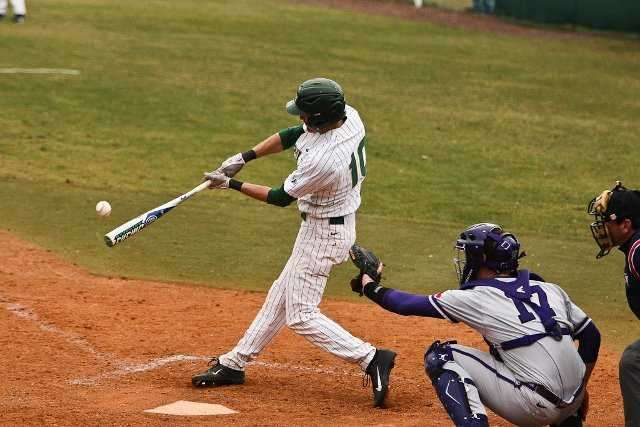
\includegraphics[width=2.0in]{images/ab.jpg}
\end{figure}
\end{column}%
\hfill%
\begin{column}{.48\textwidth}

\beqn
BA := \frac{\# \text{Lifetime Hits}}{\# \text{Lifetime At Bats}}
\eeqn

The \qu{:=} means \qu{defined as}.
\end{column}%
\end{columns}	
\pause



\begin{block}{\tiny Technicalities}
\begin{itemize}
\item \tiny \qu{At Bats} means every career plate appearance except walks, hit by pitch, bunts and others. \pause
\item \tiny \qu{Hits} means any career instance where they reach first base via a fair ball or home run. \pause
\end{itemize}
\end{block}

Note: detailed knowledge of baseball is not a prereq for this module, but many of the problems are motivated by baseball. 
\end{frame}

\begin{frame}
	\frametitle{Lifetime Batting Average of a Single Player}

\begin{figure}[htp]
\centering
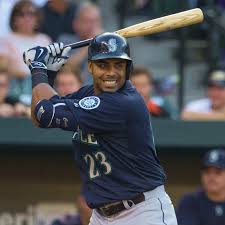
\includegraphics[width=1.0in]{images/nc.jpeg}
\end{figure}

We wish to answer three questions concerning the lifetime batting average:\pause

\begin{enumerate}
\item Given that the player has not yet retired, how do we estimate his BA? \pause
\item Provide an interval of possible BA values and assign a probability that the BA is inside that interval\pause
\item Use historical data to improve the estimates (empirical Bayes).
\end{enumerate}
\end{frame}

\begin{frame}
	\frametitle{Outline}

\begin{itemize}
\item Random Variables, the Bernoulli and Binomial simple probability models \pause
\item Parameters, Estimators and Estimates, Maximum Likelihood \pause
\item The main problem with the Frequentist Estimator\pause
\item Bayesian Machinery for the binomial likelihood model\pause
\item The Objective / Reference / Uninformative Prior\pause
\item Posterior Distribution, Bayesian Estimate, Credible Intervals \pause
\item Empirical Bayes\pause
\item Estimating Batting Averages with \texttt{R}
\end{itemize}

\end{frame}

\section{Review}

%\begin{frame}
%	\frametitle{Outline}
%
%\begin{itemize}
%\item Random Variables, the Bernoulli and Binomial simple probability models and the Central Limit Theorem
%\item \ingray{Parameters, Estimators and Estimates
%\item The main problem with the Frequentist Estimator
%\item Bayesian Machinery
%\item The Objective / Reference / Uninformative Prior
%\item Posterior, Credible Region, Posterior Predictive Distribution
%\item Empirical Bayes
%\item Estimating Batting Averages with \texttt{R}}
%\end{itemize}
%
%\end{frame}


\begin{frame}
	\frametitle{R.V. Function and the Probability Function}

\scriptsize

Technically random variables (r.v.'s) map the set of the \qu{universe} of possible \qu{outcomes} $\Omega$ \pause to a numerical outcome (a real number). \pause This is important because numerical outcomes can be modeled where non-numerical outcomes cannot be. \pause (You cannot take the average of the outcomes \qu{hit} and \qu{walk} and \qu{bunt}). \pause Here is the r.v. $X$:

\beqn
X : \Omega \rightarrow \reals
\eeqn

The \qu{support} of this random variable, $\supp{X}$ is all possible values it can \qu{spit out} i.e. the range of the function $X$. \\~\\\pause

Technically, probability is a \qu{set function} taking in \qu{events} (i.e. subsets of the universe of events and assigning an uncertainty value between 0 and 1:\pause

\beqn
\mathbb{P} : 2^\Omega \rightarrow \zeroonecl
\eeqn
\pause

\begin{block}{\tiny Technicalities}
\begin{itemize}
\item \tiny The domain is only the powerset of the universe on discrete support random variables.
\item \tiny Probability's mathematical definition is undisputed but its real-world definition is disputed by philosophers. This is beyond the scope of this module.
\item \tiny We ignore outcomes, events and the universe $\Omega$ going forward...
\end{itemize}
\end{block}

\end{frame}

\begin{frame}
	\frametitle{Model for Lifetime Batting Average}

\scriptsize 
Once again, 

\beqn
BA := \frac{\# \text{Hits}}{\# \text{At Bats}}
\eeqn\pause

Which can be thought of as:

\beqn
BA := \frac{\indic{\text{Hit 1st at bat}} + \indic{\text{Hit 2nd at bat}} + \ldots + \indic{\text{Hit $i$th at bat}} + \ldots + \indic{\text{Hit $L$th at bat}}}{1 + 1 + \ldots + 1 + \ldots + 1}
\eeqn\pause

where the \qu{indicator function} is defined as:

\beqn
\indic{\text{A}} := \begin{cases}
1 \quad\text{if event $A$ occurred} \\\pause
0 \quad\text{if event $A$ did \emph{not} occur.} \\
\end{cases}
\eeqn\pause

So if there are $L$ lifetime at bats, then the lifetime BA can be written as:\pause

\beqn
BA := \oneover{L}\sum_{i=1}^L \indic{\text{Hit $i$th at bat}}
\eeqn


\end{frame}

\begin{frame}
	\frametitle{The Bernoulli R.V.}

\scriptsize

Let's meditate on what $\indic{\text{Hit $i$th at bat}}$ really is. First of all, it can be 1 if the player got a hit on the $i$th at bat and 0 if not. And the outcome is random. \pause Let's call it $X$ and call the probability of the hit $\theta$. Thus,

\beqn
X = \begin{cases}
1 \quad\text{with probability $\theta$} \\
0 \quad\text{with probability $1 - \theta$} \\
\end{cases}
\eeqn\pause


This situation comes up a whole lot: one random \qu{trial} or \qu{experiment} and we wish to \qu{count} if the event of interest happened. \pause This is called the \qu{bernoulli r.v.} and it is denoted via:

\beqn
X \sim \bernoulli{\theta}
\eeqn

where the $\sim$ means distributed as and the $\bernoulli{\theta}$ is just shorthand for the cases \qu{1 w.p. $\theta$ and 0 otherwise}. \\~\\\pause

What is $X$ exactly? It's a \qu{probability model} for a future outcome, $x$. Note the capital letter and lowercase letter. The future outcome is also called a \qu{realization} because the model gets \qu{realized} (i.e. made to be real) when the random trial is completed. \\~\\\pause

What is $\supp{X}$? Since the only two legal things that could happen are the hit (1) and not a hit (0), $\supp{X} = \braces{0, 1}$. 

\end{frame}

\begin{frame}
	\frametitle{Probability Mass Function (PMF)}

\scriptsize 
The r.v. can be entered into the probability function to query the outcome of the experiment. For instance, what is:

\beqn
\prob{X = 1} &=&\pause \theta \\
\prob{X = 0} &=& \pause 1 - \theta
\eeqn

These may seem like simple questions, but ponder the following, what if we index the realization by the free variable $x$  and ask the question. \pause

\beqn
\prob{X = x} = \theta^x (1-\theta)^x := \prob{X}\pause
\eeqn

This is an important function, it is called the \qu{probability mass function} (PMF) and we'll denote it $\prob{X}$. We will also call this its \qu{density}. It has the property that $\sum_{x \in \supp{X}} \prob{x} = 1$. \pause

\begin{block}{\tiny Technicalities}
\begin{itemize}
\item \tiny The domain of the probability function is a subset of $\Omega$, so technically the first query $\prob{X = 1} $ is an \qu{abuse of notation} which is \qu{shorthand} for $\prob{\braces{\omega \in \Omega : X(\omega) = 1}} = \prob{\braces{\omega = \text{Hit}}} = \theta$.
\item \tiny $x$ can take on only those values $\in \supp{X}$. In the above, any value $\notin \supp{X}$ gets probability 0. So e.g. $\prob{X = 17} = 0$ and $\prob{X = \frac{2}{3}} = 0$, etc.
\item Densities are only available for continuous r.v.'s (which we will see later in this module)
\end{itemize}
\end{block}

\end{frame}

\begin{frame}
	\frametitle{Detour: Continuous Random Variables}

If a r.v. (not the bernoulli r.v.) has a support that is not countably infinite (e.g. $\braces{1,2, \ldots}$), \pause then that r.v. is called \qu{continuous}. \pause A few properties:

\begin{itemize}
\item These r.v.'s do not have PMF's, they have \qu{probability densitity functions} (PDF's) which we will also denote $\prob{X}$. \pause
\item All probabilities of individual values is zero i.e. $\prob{X = x} = 0$ for all values of $x$. \pause
\item Probabilities are calculated only over a range via the following integration:

\beqn\label{eq:pdf_prob}
\prob{a \leq X \leq b} = \int_a^b \prob{X} dx \quad \text{and thus} \quad \int_{x \in \supp{X}} \prob{X} dx = 1
\eeqn \pause

\begin{block}{\tiny Technicalities}
\tiny Usually, the PMF and PDF are given different notation $p(x)$ and $f(x)$. We are calling them both $\prob{X}$ here for simplicity as they will be both used within the Bayesian paradigm interchangably --- this is a slight abuse of notation as sometimes you will not know if the r.v. is discrete or continuous from its notation.
\end{block}

\end{itemize}


\end{frame}

\begin{frame}
	\frametitle{Detour: Expectation of Random Variables}

\scriptsize

Random variables have a \qu{balancing point} of their support. \pause It is similar to how the \qu{center-of-mass} is calculated in physics. \pause We call this quantity the \qu{expectation} or \qu{mean} and denote it $\expe{X}$ and calculate it via: \pause

\beqn
\expe{X} &=& \sum_{x \in \supp{X} } x~ \prob{X = x} \eqncomment{for non-continuous r.v.'s} \\ \pause
\expe{X} &=&  \int\limits_{ x \in \supp{X} } x ~\prob{X = x} dx \eqncomment{for continuous r.v.'s} \\ \pause
\eeqn

For example, the expectation of the bernoulli r.v. would be:\pause

\beqn
\expe{X} &=& \pause \sum_{x \in \supp{X} } x \prob{X = x} = \pause \sum_{x \in \braces{0, 1}} x \theta^x (1-\theta)^{1-x} \\ \pause
&=& (0) \theta^0 (1-\theta)^{1-0} + (1) \theta^1 (1-\theta)^{1-1} = \pause \text{\fbox{$\theta$}} \pause
\eeqn



\begin{block}{\tiny Technicalities}
\tiny In general, the expectation is not a parameter alone but a function of the parameter(s). Bernoulli is a special case in this regard. \pause
\end{block}

Back to our regularly scheduled program...

\end{frame}

\begin{frame}
	\frametitle{Parameter}

But conceptually, what is $\theta$? \pause This quantity is known as a \qu{parameter}. \pause The exact value of a parameters is unknowable with finite data. \pause In classical statistics, we provide \qu{inference} which is loosely, \pause

\footnotesize

\begin{enumerate}
\item estimate its value\pause
\item form a hypothesis of its value and then test the hypothesis (experimentation) \\~\\\pause


Using the Bayesian outlook, one can do the above and more, \\~\\

\item find the density of $\theta$ \pause
\item use historical data to improve the estimation
\end{enumerate}

We will be covering 1, 3 and 4.
\end{frame}

\begin{frame}
	\frametitle{Our Parameter of Interest}

But what is $\theta$ in our problem? \pause Remember, if $X_i$ represents the player of interest's $i$th at bat,

\beqn
X_i \sim \bernoulli{\theta} := \pause \begin{cases}
1 \quad\text{if he got a hit on his $i$th at bat} \\ \pause
0 \quad\text{if he did not get a hit on his $i$th at bat}
\end{cases}
\eeqn \pause

This means $\theta$ is the true probability of the $i$th at bat. \pause Since we only observe $x_i = 1$ or $x_i = 0$, you can intuitively see how $\theta$ can never be known \pause --- not enough information to determine it. \\~

What values can $\theta$ be? \pause We say $\theta \in \Theta$ which is its \qu{parameter space}. Since $\theta$ is a probability, all values between 0 and 1 are allowed. \pause But to keep the problem non-trivial, we do not allow 0 or 1, and thus we have

\beqn
\theta \in (0, 1) \quad \text{which is the \qu{parameter space} of the Bernoulli r.v.}
\eeqn

\end{frame}

\begin{frame}
	\frametitle{Identically Distributed}

The next concept is subtle. Let's consider the first at bat and the second at bat: $X_1$ and $X_2$. \pause  It could be there are different probabilities of getting hits. Why? One day the player is on his game and the next day he's off his game, thus:\pause 

\beqn
X_1 \sim \bernoulli{\theta_1}, \quad X_2 \sim \bernoulli{\theta_2} ~~s.t.~~ \theta_1 > \theta_2
\eeqn

In which case we would be estimating two different parameters! \pause Taken to the extreme, when examining $n$ hits, there would be $n$ different parameters. So we make a simplifying assumption: we pretend the player has \qu{one true} probability of getting a hit, which we call $\theta$ and hence $X_1$ and $X_2$ share that same $\theta$ and are thus identically distributed. \pause \emph{We now assume (which will be slightly modified later) that $X_1, \ldots, X_n$ are identically distributed.}

\end{frame}

\begin{frame}
	\frametitle{Detour: Conditional Probability}

Another subtle concept. Let's consider the following question: if you know the player got a hit on the first at bat, would that change the probability of getting a hit the next at bat? \pause If the answer is that the probability would go up, this is known as \qu{hitting streak} in baseball. \pause  In our notation this would be:

\beqn
\cprob{X_2 = 1}{X_1 = 1} > \prob{X_2 = 1}
\eeqn

You may remember the l.h.s.'s notation with the vertical line symbol (the \qu{pipe}) is known as \qu{conditional probability} \pause and the notation on the right --- the \qu{default} probability notation --- is known as an \qu{unconditional probability}. \pause In our case, knowing that there was a hit just before this at bat (i.e. that $X_1 = 1$) makes the second at bat more likely to result in a hit than if you didn't have the previous information (just the r.h.s.).

\end{frame}

\begin{frame}
	\frametitle{Definition of Conditional Probability}

\scriptsize
How do we define conditional probability? Two images are  below. \pause 

\begin{columns}[T] % align columns
\begin{column}{.48\textwidth}
\begin{figure}
\centering
\fbox{
\includegraphics[width=1.0in]{images/smallbug.jpeg}}
\end{figure}
\end{column}%
\hfill%
\begin{column}{.48\textwidth}
\begin{figure}
\centering

\includegraphics[width=1.0in]{images/magn.jpeg}
\end{figure}
\end{column}%
\end{columns}	~\\



Define the event $A$ as you throw a pin on the left image and you hit the bug. \pause Safe to say $\prob{A}$ is small. \pause Now imagine you throw a pin inside the field of the magnifying glass on the right. Safe to say $\prob{A}$ is large there. \\~\pause 

But they're not the same events! Consider the event $B$ where you have the magnifying glass. Pinning the bug, $A$, while you have $B$ raises the probability of $A$, thus\pause 

\beqn
\cprob{A}{B} > \prob{A}.
\eeqn

\end{frame}

\begin{frame}
	\frametitle{Bayes Rule}

By how much is $\cprob{A}{B}$ bigger than $\prob{A}$? \pause The bug on the right is in intersection of $A$ and $B$ at the same time. The zoom factor is whatever the original size of the field was (the box from the left image) divided by the new size. On the left, the whole box has probability 1 since it represents the universe. So the zoom factor is $\oneover{\prob{B}}$. \pause Thus,

\beqn
\cprob{A}{B} = \underbrace{\prob{AB}}_{\text{original size of bug}} \times \underbrace{\oneover{\prob{B}}}_{\text{zoom factor}} = \frac{\prob{AB}}{\prob{B}}
\eeqn

This rule is known as \emph{Bayes Rule} \pause and it will form the basis for what we do in the next unit. \pause 


\begin{block}{\tiny Technicalities}
\tiny This example is a bit confusing. Here, $AB = A$ since $A$ is a proper subset of $B$.  The original bug size is $A$ which is also $AB$. Thus, $\cprob{A}{B} = \prob{A} / \prob{B}$ only in this case though.
\end{block}

\end{frame}


\begin{frame}
	\frametitle{Independence}

So now that we know what conditional probability is, let's return to the two at bats, $X_1$ and $X_2$. \pause  Imagine if knowing what happened at the first at bat $X_1$ did not inform anything about $X_2$. \pause  Then the conditional and the unconditional would be one and the same:

\scriptsize
\beqn
\cprob{X_2 = x_2}{X_1 = x_1} = \prob{X_2 = x_2} \quad \text{and shorthand,} \quad \cprob{X_2}{X_1} = \prob{X_2}
\eeqn
\normalsize\pause 

This is known as \qu{independence}. \\~

Via Bayes Rule, we have:\pause 

\beqn
\cprob{X_2}{X_1} = \frac{\prob{X_1, X_2}}{\prob{X_1}} = \prob{X_2} \Rightarrow \prob{X_1, X_2} = \prob{X_1}\prob{X_2}
\eeqn\pause 

So independence implies that joint events factor and you can multiply them. \pause  \emph{We now assume (which will be slightly modified later) that $X_1, \ldots, X_n$ are independent.} 

\end{frame}

\begin{frame}
	\frametitle{IID and Total Hits}

We say that the r.v.'s are IID and denoted $\Xoneton \iid \bernoulli{\theta}$ \pause if we have the situation where the probability that any of the at bats will yield a hit is the same, $\theta$ (identical distribution) and that knowing any of the outcomes of the at bats does not affect any other hit at any other at bat (independence). \\~\pause 

Now consider tallying all the hits in $n$ at bats. This would be equivalent to the sum of all the $X_i$'s since we only care about summing the 1's, call this $X$ (even though it's confusing), \pause 

\beqn
X = \sum_{i=1}^n X_i
\eeqn

Can we find the PMF of $X$? \pause Can we ask what is the probability of yea so many hits out of $n$?

\end{frame}

\begin{frame}
	\frametitle{The PMF of the sum of Bernoullis}

\scriptsize
Imagine for a moment there are $n=6$ at bats \pause and the probability of a hit $\theta = 0.25$. \pause  How could we find the probability of 3 hits out of 6 at bats i.e. $\prob{X=3}$? \\~\pause 

Denote hit as $H$ and not hit as $O$. There are 20 ways to make 3 hits occur out of 6:\pause 

\beqn
HHHOOO \quad HHOHOO \quad HOHHOO \quad OHHHOO \\
HHOOHO \quad HOOHHO \quad OOHHHO \quad HHOOOH \\ 
HOOOHH \quad OOOHHH \quad HOOHOH \quad HOHOOH \\ 
HOHOHO \quad OHOHOH \quad OHHOHO \quad OOHHOH \\ 
OOHOHH \quad OHHOHO \quad OHHOOH \quad OHOOHH \\ 
\eeqn\pause 

Since each string of H's and O's is independent, \pause the probability of each will always be $0.25^3 0.75^3$ \pause since each the probability of each at bat can be multiplied. \pause So now we need to count the number of ways to make 3 H's in 6 positions. \pause Recall from basic probability that this is $\binom{6}{3} = \frac{6!}{3! (6-3)!} = 20$. So, \pause 

\beqn
\prob{X=3} = \binom{6}{3} 0.25^3 0.75^3 = \texttt{dbinom(3, 6, 0.25)} \approx 0.132
\eeqn\pause 

Where \qu{\texttt{dbinom(3, 6, 0.25)}} is the \texttt{R} code to compute the answer. 
\end{frame}

\begin{frame}
	\frametitle{The Binomial Model}

Again consider $n$ at bats with arbitrary probability of a hit $\theta$ (which is limited by its parameter space). \pause  The r.v. we spoke about is actually called the binomial r.v.,

\beqn
X_n = \sum_{i=1}^n X_i \sim \binomial{n}{\theta}
\eeqn\pause 

Its PMF can be found by generalizing the reasoning from the last slide:\pause 

\beqn
\prob{X=x} = \binomial{n}{\theta} := \binom{n}{x} \theta^x (1-\theta)^{n-x}
\eeqn


\end{frame}


\begin{frame}
	\frametitle{The Role of Data}

Given that we have $n$ at bats and we assume each at bat is an $\iid$ bernoulli with parameter $\theta$, \pause we now focus on estimating $\theta$ and testing ideas about $\theta$. \\~\\\pause 

To do so, we use \emph{data} to estimate $\theta$ and in our case, that's just $x_1, x_2, \ldots, x_n$ which looks like a string of $n$ 0's and/or 1's. \pause 

\begin{block}{\tiny Technicalities}
\tiny $\theta$ isn't exactly the lifetime batting average, it's deeper: it's the intrinsic propensity for the batter under scrutiny to create a hit out of an at-bat. If the number of lifetime at-bats is large, the lifetime BA and $\theta$ will be quite similar. We will ignore this detail.
\end{block}\pause 

So how do we use data? \pause We first begin with the popular tools of frequentist estimation and then move to the Bayesian tools which is the focus of this module.

\end{frame}


\begin{frame}
	\frametitle{Homework Problems}
\begin{enumerate}
\item[1] Draw the PMF for $X \sim \bernoulli{\theta}$. 
\item[2] Imagine two Bernoulli r.v.'s $X_1$ and $X_2$ which model two fair coin flips where Heads is mapped to 1 and tails is mapped to 0. The probability of heads is 1/2. Explain using the definition of r.v. independence why these two r.v.'s are \textit{dependent}.
\item[3] Using the same two sorcery-controlled coins, explain using the definition of equality in distribution why or why not $X_1$ and $X_2$ are equally distributed.
\item[4] Are $X_1, X_2 \iid \bernoulli{\theta}$ if they are modeled by these two sorcery-controlled coins?
\item[5] A new situation: the probability of a bundle of coins (scotch-taped together) landing on its side is $\prob{S} = 1/11$. Heads and tail probability are 5/11. Let's call landing on its side the event we seek, create a Bernoulli r.v. for this event indicate its support, its parameter and the parameter space.
\end{enumerate}
\end{frame}	

\begin{frame}
	\frametitle{Homework Problems}
\begin{enumerate}

\item[6]  I flip the coin bundle once. What is the probability of the trial of interest being found? Write a probability statement.
\item[7]  Let's say we flip 10 times. What is the probability that we get one (and only one) success? I want to see a probability model.  Write \qu{$X \sim$} something below. Then I want to see a probability statement. Then I want to see a computation. Answer then in decimal rounded to two digits. 
\item[8] Let's say we flip 10 times. What is the probability that we get 5 (and only 5) successes?  
\item[9]  Let's say we flip 10 times. What is the probability that we get 8 (and only 8) successes?  
\item[10] Let's say we flip 10 times. What is the probability we get one or two successes?  

\end{enumerate}
\end{frame}	

\begin{frame}
	\frametitle{Homework Problems}
\begin{enumerate}

\item[11]  Consider three NYC buildings: One World Trade Center (104 floors), the Empire State Building (86 occupied floors) and the Bank of America Tower (55 floors). Consider walking into one of them at random and picking a random floor. What is the probability of choosing the Empire State Building's 40th floor?
\item[12] What is the probability he on the 30the floor?
\item[13] If you know he's on the 40th floor, what is the probability he is in the empire state building?
\item[14] Look up the Monte Hall game. Explain why switching is a good strategy based on conditional probability.
\item[15] Is the $\iid$ bernoulli model for at bats a good model in baseball? This is complicated.
\end{enumerate}
\end{frame}	


\section{Frequentist Estimation}

\begin{frame}
	\frametitle{Likelihood function}

\scriptsize
Recall from before the PMF for our data (which is a function of the free variable $X$),

\beqn
\prob{X; \theta} = \binom{n}{x} \theta^x (1-\theta)^{n-x}.
\eeqn\pause 

I've wrote it differently. Here I use $\theta$ as information you need to calculate the function. \pause 

\begin{block}{\tiny Technicalities}
\tiny This is similar to the following polynomial: $f(x; a) = ax^2$. \\~\\

Here, $a$ is not to be considered a second free variable in the function, but a constant tuning parameter which provides customization for the shape of the parabola (thin to fat and everything in between). This is exactly what $\theta$ does above.
\end{block}\pause 

What if we \qu{flip} or invert the role of the data and the parameter? We still get the same thing, but I'll use different notation:

\beqn
\lik{\theta; X} = \binom{n}{x} \theta^x (1-\theta)^{n-x}.
\eeqn\pause 

The $L$ stands now for likelihood and the $\theta$ is now the free variable and the data $X$ is the parameter. (but otherwise it is the same as the PMF!)

\end{frame}

\begin{frame}
	\frametitle{Maximum Likelihood and the MLE}

\scriptsize
Why did we do this? \pause Because we now can ask the question: which value of $\theta$ is the \emph{most likely} for this data. \pause  We call this the maximum likelihood estimator (MLE):\pause 

\beqn
\thetahatmle := \argmax_{\theta \in \Theta} \lik{\theta; X}
\eeqn\pause 

This comes down to taking the derivative, \pause setting it equal to zero and solving for $\theta$ just like in Calculus 101. \pause Note that the maximum of the function is immune to monotonic transformations of the function. \pause One such convenient monotonic transformation is the natural log, $\loglik{\theta; X} := \natlog{\lik{\theta; X}}$, \pause so we can now calculate the maximum likelihood estimator via\pause 

\beqn
\thetahatmle := \argmax_{\theta \in \Theta} \loglik{\theta; X}
\eeqn\pause 

and that will be our definition going forward. \pause  So let's begin solving for the MLE of $\theta$ given our data from $n$ at bats:\pause 

\beqn
&& 0 \pause \seteq \pause \partialop{\theta}{\loglik{\theta; X}} = \pause \partialop{\theta}{\natlog{\binom{n}{X}} + X \natlog{\theta} + (n-X) \natlog{1-\theta}} = \pause \frac{X}{\theta} - \frac{n-X}{1-\theta} \\\pause 
&& \Rightarrow (1-\theta)X = \pause \theta(n-X) \Rightarrow X - \cancel{x\theta} = \pause n\theta - \cancel{X\theta} \Rightarrow \thetahatmle \pause = \overn{X}
\eeqn

\end{frame}

\begin{frame}
	\frametitle{The Sample Average}

\scriptsize
If you recall, $X$ was defined as the sum of Bernoulli r.v.'s, \pause  hence we can rewrite the MLE as:

\beqn
\thetahatmle = \overn{X} = \overn{ \sum_{i=1}^n X_i} = \Xbar
\eeqn\pause 

This is the \emph{estimator} (the r.v. that represents how the estimate is drawn). \pause To find the maximum likelihood \emph{estimate} you can plug in the data into the estimator:\pause 

\beqn
\thetahatmle = \overn{x} = \overn{ \sum_{i=1}^n x_i} = \xbar
\eeqn\pause 

Note how everything is lowercase now. \pause  But through an abuse of notation, I didn't change the notation $\thetahatmle$. \pause But more importantly --- you've seen this before! \\~\\\pause 

Remember adding up all the numbers and then dividing by the number of numbers from high school? This is called the \qu{sample average}. \pause  (In the our special case of the binomial $\theta$ estimation, you may see it written as $\hat{p}$ instead). \\~\\\pause 

This is our best guess as to the value of $\theta$. 

\end{frame}

\begin{frame}
	\frametitle{Trouble with the Sample Average}

\scriptsize
So if there were 100 at bats and 29 hits, the batting average is 0.290 and that is our best guess as to the true propensity of the batter to get a hit. \pause  So computing the BA is a good idea!! \\~\\\pause 

But what if there were two at bats and there were no hits? Or two hits? \pause 

\beqn
\xbar = \frac{0}{2} = 0.000, \pause \quad\xbar = \frac{2}{2} = 1.000 
\eeqn\pause 

All these batting averages are absurd!  Why? \pause 

\begin{enumerate}\scriptsize
\item The first says he will never make a hit. Well why is he paid millions of dollars then? This estimate is clearly off. \pause 
\item The second says he will always make a hit. That is clearly wrong. \pause 
\end{enumerate}

The \qu{Frequentist} view forces us to be purely \qu{objective} and let the data (and only the data) speak on behalf of the underlying unknown parameter. \pause  But this is clearly silly sometimes!

\end{frame}



\begin{frame}
	\frametitle{Homework Problems}
\begin{enumerate}
\item[1] Rederive the MLE (estimator and estimate) for the Binomial likelihood model.
\item[2] Try to derive it without using the monotonic transformation of the log of the likelihood.
\item[3] Instead of the maximum likelihood, write an expression for the 90\%ile of the likelihood.
\item[4] Given 345 at bats and 132 hits, what is the maximum likelihood of the hit probability?
\item[5] Is $\theta$ the same as lifetime batting average? Discuss.
\item[6] Why is an MLE of 0.000 or 1.000 a bad thing? Discuss.
\item[7] Devise a means to fix these two pathological situations without looking ahead in the module.
\end{enumerate}
\end{frame}	

\section{Bayesian Estimation}

\begin{frame}
	\frametitle{Introduction}

How do we solve this problem of 0.000 and 1.000 batting average estimates? \pause  Bayesian statistics is one approach we will explore here. \\~\\\pause 

\emph{The Bayesian Paradigm Shift} \\ ~ \\

Imagine that $\theta$ is still a single value still unknown, \pause but now we are able to quantify our uncertainty about where $\theta$ is using a distribution, $\prob{\theta}$. \pause Now, $\theta$ becomes its own r.v! \pause  We are interested in what happens to this uncertainty with the introduction of data ($X$), \pause 

\beqn
\theta \quad \buildrel data \over \longrightarrow \quad\theta~|~X
\eeqn

This is called \qu{Bayesian Conditionalism}. \pause We begin with what is called the \qu{prior} and we update it to find the \qu{posterior} --- data is able to refine our ideas about where $\theta$ is likely to be.

\end{frame}

\begin{frame}
	\frametitle{Bayes Rule Again}

\scriptsize
How does this update work? \pause  Through Bayes Rule! \pause 

\beqn
\underbrace{\cprob{\theta}{X}}_{\text{posterior}} \pause = \frac{\prob{X, \theta}\pause }{\prob{X}} = \pause  \underbrace{\frac{\cprob{X}{\theta}}{\prob{X}}}_{\text{update factor}}\pause  \underbrace{\prob{\theta}}_{\text{prior}}
\eeqn

The l.h.s. is a density for $\theta$ under your data. \pause You can query it with ideas about what you think $\theta$ is and it returns probabilities (or probability densities). \pause The update factor is how likely the data is under an idea of $\theta$ out of all possibilities for $X$. \pause  If the data supports a given $\theta$, then the update factor is greater than 1, otherwise less than 1. \pause  Note that the update factor is the likelihood $\cprob{X}{\theta}$ divided by $\prob{X}$, a term called the \qu{prior predictive distribution} which we will not focus on too much (you'll see why later). \pause 

\begin{block}{\tiny Technicalities}
\tiny Previously we defined likelihood as $\prob{X; \theta}$ but now it's $\cprob{X}{\theta}$. \pause Why did the semicolon become a pipe character? \pause Previously $\theta$ was considered a fixed constant, a parameter in the function. But now it is its own random variable with full-citizen rights! \pause We thereby give it a true pipe character.
\end{block}\pause 

Note that the posterior is \qu{given $X$}. \pause  We will return to this shortly after we speak about kernels.

\end{frame}


\begin{frame}
	\frametitle{Review: What is a kernel?}

\scriptsize

Recall from your probability class that a PMF (or PDF) sums (or integrates) to 1. \pause Thus if they're multiplied by a constant $1/c$, they'll sum (or integrate) to $1/c$. \pause For instance the binomial PMFs sums to 1,

\beqn
\sum_{x=0}^n \prob{X} = \sum_{x=0}^n \frac{n!}{x! (n-x)!} \theta^x (1-\theta)^{n-x} = 1
\eeqn\pause 

but the following quantity is equal to $1/n!$, \pause 

\beqn
\sum_{x=0}^n \frac{1}{x! (n-x)!} \theta^x (1-\theta)^{n-x} = 1/n!
\eeqn

Since $1/n!$ is not a function of the free variable $x$, we say that\pause 

\beqn
\frac{1}{x! (n-x)!} \theta^x (1-\theta)^{n-x} \propto \prob{X}
\eeqn\pause 

The \qu{proportionality} sign indicates it differs from the true PMF by only a constant which can be recovered by doing the sum.

\end{frame}



\begin{frame}
	\frametitle{Review: What is a kernel?}

\scriptsize

We can go further and remove all constant multiples that do not depend on $x$ to obtain the \qu{kernel} which we'll denote $k(x)$, \pause 

\beqn
k(x) := \frac{1}{x! (n-x)!} \tothepow{\frac{\theta}{1 - \theta}}{x}\propto \prob{X}
\eeqn\pause 

Kernels are interesting... if we find them, we have quantity proportion to $\prob{X}$ and therefore we know it is the same as the true PMF. \pause So if you see $k(x)$ above you know $X \sim \binomial{n}{\theta}$! \pause They also can be used to calculate proportions of probabilities:

\beqn
\frac{k(a)}{k(b)} = \frac{\prob{X = a}}{\prob{X = b}}
\eeqn\pause 

since the constant will cancel. \\~\\\pause 
%HW kernel of all the PMFs

Now let's return to Bayes Rule, note that:

\beqn
\cprob{\theta}{X} = \frac{\prob{X, \theta}}{\prob{X}} =  \frac{\cprob{X}{\theta}}{\prob{X}} \prob{\theta} \propto\pause  \cprob{X}{\theta} \prob{\theta} = \pause \text{likelihood} ~\times~ \pause \text{prior}
\eeqn\pause 

(since $1/\prob{X}$ is clearly a constant and not a function of the free variable $\theta$).

\end{frame}

\begin{frame}
	\frametitle{The prior}

\scriptsize
We know what the likelihood is from before, but what is the prior? \pause $\prob{\theta}$ is your belief over all $\theta$ of what $\theta$ is before you see data. \pause This is a weird concept! So let's \qu{break it in slowly}. \pause  First of all, what could $\theta$ be in our batting average problem? It's the probability of getting a hit, the parameter in the underlying Bernoulli. \pause  It should be fair to say that every possibly parameter value should be represented in a prior, thus\pause 

\beqn
\supp{\theta} = \text{the parameter space of the Bernoulli}
\eeqn 

which is a link between parameter spaces and supports. \\~\\\pause 

Now if we want to be as \qu{objective} as possible or to be as \qu{uninformative} or as \qu{indifferent} as possible, we can use a \qu{uniform} prior (also called a \qu{reference} prior). \pause This is five names for the same thing:

\beqn
\prob{\theta} = \uniform{0}{1} = \begin{cases}
1 \quad\text{if} \quad \theta \in \zeroonecl \\
0 \quad\text{otherwise}
\end{cases}
\eeqn\pause 

This means no matter what the value of $\theta$, we don't think any of them are more likely than any other!

\end{frame}

\begin{frame}
	\frametitle{Posterior Kernel}

\scriptsize
Previously we showed that $\cprob{\theta}{X} \propto \cprob{X}{\theta} \prob{\theta}$. \pause With the uniform prior we just discussed, $\prob{\theta} = 1$. \pause This means that $\cprob{\theta}{X} \propto \cprob{X}{\theta} (1)$ and for our binomial likelihood model, \pause 

\beqn
\cprob{\theta}{X} \propto \binom{n}{x} \theta^x (1-\theta)^{n-x}
\eeqn\pause 

Since we are given the data $X$ and we know $n$ as well by assumption, \pause  we can make the kernel a bit tighter:

\beqn
\cprob{\theta}{X} \propto \theta^x (1-\theta)^{n-x} := k(\theta~|~X)
\eeqn\pause 

We know that $k(\theta~|~X)$ must correspond to a density of $\theta$ which is a constant $c$ times the kernel. To find its constant, we integrate over the parameter space, \pause 

\beqn
\oneover{c} := \int\limits_{\theta \in \zeroonecl} \theta^x (1-\theta)^{n-x} dx
\eeqn\pause 

This is a very famous integral! \pause It is known as the beta integral and its solution is the non-computable (but approximable) beta function.

\end{frame}


\begin{frame}
	\frametitle{The Beta Function}
	
The beta function is:

\beqn
B(\alpha, \beta) := \int_0^1 t^{\alpha - 1} (1-t)^{\beta - 1} dt
\eeqn\pause 

So the integral from the previous page becomes:

\beqn
B(x + 1, n - x + 1) =  \int\limits_{\theta \in \zeroonecl} \theta^x (1-\theta)^{n-x} dx
\eeqn\pause 

and thus the density becomes (since the l.h.s is $1/c$),

\beqn
\cprob{\theta}{X} = \oneover{B(x+1, n-x+1)} \theta^x (1-\theta)^{n-x}
\eeqn 

\end{frame}


\begin{frame}
	\frametitle{The Beta Distribution}

\scriptsize
Just like the beta function, this is the density of a famous continuous r.v. called the \qu{beta},

\beqn
Y \sim \stdbetanot := \oneover{B(\alpha, \beta)} y^{\alpha - 1} (1-y)^{\beta - 1}
\eeqn\pause 

where $\supp{Y} = (0, 1)$ \pause and the parameter space is $\alpha > 0$ \pause and $\beta > 0$. \pause Since there are two parameters, there are many different shapes this can look like: \pause 

\begin{figure}
\centering
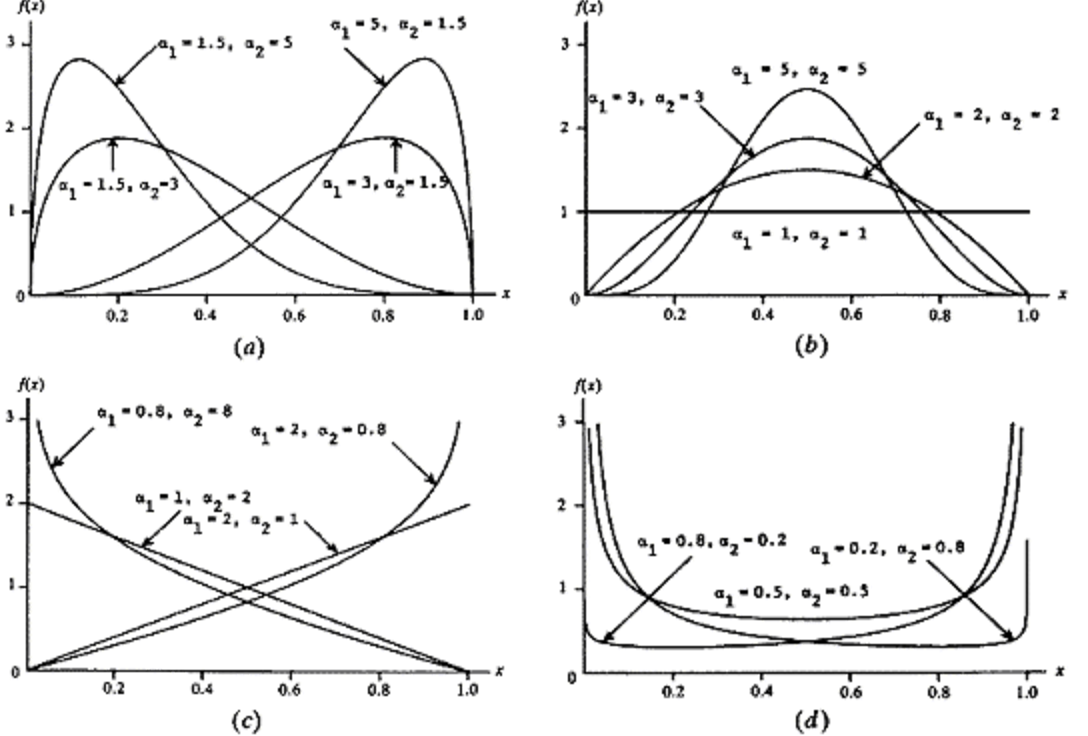
\includegraphics[width=2in]{images/betadist.png}
\end{figure}\pause 

So, now we have moved from $\theta \sim U(0,1) \rightarrow$ \pause $ \theta~|~X \sim \betanot{x+1}{n-x+1}$ using Bayesian conditionalism.

\end{frame}


\begin{frame}
	\frametitle{Posterior --- what is it?}
	
So we have the posterior. What can we do with it? \pause Anything you want! \pause What if you want to know the probability the batting average is under 200? \pause Then,

\beqn
\cprob{\theta \leq 0.2}{X} = \int\limits_{0}^{0.2} \oneover{B(x+1, n-x+1)} \theta^x (1-\theta)^{n-x} d\theta
\eeqn\pause 

where the integral can be figured out by numerical integration using \texttt{R} via the command \texttt{pbeta(0.2, x+1, n-x+1)}. \pause Any probability can now be queried about $\theta$! \pause This was not possible with the frequentist / classical approach.

\end{frame}

\begin{frame}
	\frametitle{Bayesian Estimate}

\scriptsize
We have the whole distribution $\cprob{\theta}{X}$ but what if you were forced to give one answer as to your best guess of $\theta$. \pause Recall the MLE was

\beqn
\thetahatmle = \xbar = \frac{x}{n}
\eeqn\pause 

But what do we do with a whole distribution? \pause What is the best guess? \pause Why not what the average guess is? That's what the expectation is, so let's compute the expectation for the beta density, \pause 

\beqn
\expe{Y} &=& \pause \int\limits_0^1 y \oneover{B(\alpha, \beta)} y^{\alpha - 1} (1-y)^{\beta - 1} dy \\
&=& \pause \oneover{B(\alpha, \beta)}  \int\limits_0^1 y^{\alpha} (1-y)^{\beta - 1} dy \\
&=& \pause \frac{B(\alpha -1, \beta)}{B(\alpha, \beta)} =\pause  \frac{\alpha}{\alpha + \beta}
\eeqn

where the last equality is due to the beta function being expressible as the gamma function \pause and properties of the gamma function.
\end{frame}


\begin{frame}
	\frametitle{The Posterior Expectation}
	
Thus in our setup, with $\theta \sim \stduniform$, our Bayesian estimate, using the posterior expectation we just derived, is\pause 

\beqn
\cexpe{\theta}{X} = \frac{(x + 1)}{(n - x + 1) + (x + 1)} = \frac{x+1}{n+2}
\eeqn\pause 

which is called the \qu{Bayes-Laplace rule inverse probability}. \pause Note that this is very similar to the MLE, $\frac{x}{n}$. \pause 


\begin{block}{\tiny Technicalities}
\tiny There are other Bayesian estimates regularly in use which we won't discuss further. \pause
\begin{itemize}
\item \tiny The maximum a posteriori i.e. the mode of the posterior is $\argmax_\theta \braces{\cprob{\theta}{X}}$ \pause 
\item \tiny The minimum absolute error i.e. the median of the posterior \pause
\end{itemize}
\tiny We use the posterior expectation because it minimizes the squared error loss from the truth $\theta$ and this is usually an appropriate loss function unless there are other considerations.
\end{block}

\end{frame}

\begin{frame}[fragile]
	\frametitle{Credible Intervals}

What if we don't need a single point estimate but instead want the equivalent of the 95\% confidence interval? \pause We want to provide an interval of possible $\theta$ values where there is 95\% probability the true $\theta$ resides inside.  \pause The easiest way to do this is to use the posterior and return the 2.5\% quantile and the 97.5\% quantile (i.e. the \qu{middle} 95\% of the distribution) via a numerical solver algorithm. \pause This can be done in \texttt{R} via the following commands:

\begin{verbatim}
qbeta(0.025, x + 1, n - x + 1)
qbeta(0.975, x + 1, n - x + 1)
\end{verbatim}


\end{frame}

\begin{frame}
	\frametitle{The Beta Prior}

\scriptsize	
Note that our prior, $\theta \sim U(0, 1)$ can be thought of as

\beqn
\theta \sim \betanot{1}{1} \pause = \oneover{B(1,1)} \theta^{1 - 1} (1-\theta)^{1-1} \pause = \oneover{(1)} (1)(1) = 1 \pause \equalsindist U(0,1)\pause 
\eeqn

Could it be the we can generalize our prior to a beta and thereby have more \qu{options} than just a $U(0,1)$? \pause  Let's see, let's let $\theta \sim \betanot{\alpha}{\beta}$, \pause 

\beqn
\cprob{\theta}{X} &\propto& \cprob{X}{\theta} \prob{\theta} \\\pause 
&\propto& \parens{\binom{n}{x} \theta^{x} (1-\theta)^{n-x}} \pause \parens{\oneover{B(\alpha, \beta) \theta^{\alpha - 1} (1-\theta)^{\beta - 1}}} \\\pause 
&\propto&  \theta^{x} (1-\theta)^{n-x}  \theta^{\alpha - 1} (1-\theta)^{\beta - 1} \\\pause 
&=& \theta^{x + \alpha - 1} (1-\theta)^{n-x + \beta - 1} \\
\eeqn

Where this is now the kernel of the beta! \pause So,

\beqn
\theta~|~X \sim \betanot{x + \alpha}{n - x + \beta}
\eeqn

\end{frame}


\begin{frame}
	\frametitle{Beta is the \qu{Conjugate Prior}}
	
\scriptsize
If we have the likelihood be a binomial \pause and the prior, a beta, \pause then the posterior is also a beta! \pause This is known as \qu{conjugacy} and we say \qu{the beta is the conjugate prior for the binomial model}. \pause  Although priors are still arbitrary, this gives us a feeling of \qu{naturalness} about having the beta prior. \\~\\\pause 

Then we have two choices to make, what is $\alpha$ and what is $\beta$ in the prior? \pause (Under the uniform, $\alpha = 1$ and $\beta = 1$ but now we are generalizing this). \pause  Let's take a look at the Bayesian point estimate, the posterior expectation, \pause 

\beqn
\cexpe{\theta}{X} = \frac{x + \alpha}{n + \alpha + \beta} \pause \neq  \frac{x}{n} = \thetahatmle
\eeqn\pause 

Here, $\alpha$ can be interpreted as the \qu{pseudocount} number of previous hits \pause in a pseudocount number of at-bats $\alpha + \beta$. \pause  If we don't have any \qu{prior information} we have $\alpha = 0$ and $\beta = 0$ and we get back the MLE. \pause This is known as the \qu{Haldane Prior} \pause and it is \qu{improper} \pause since $\alpha = 0$ and $\beta = 0$ are not technically in the parameter space of the beta density. \pause Note that whatever prior we pick, as long as $n \rightarrow \infty$, $\displaystyle \lim_{n \rightarrow \infty} \cexpe{\theta}{X} = \thetahatmle$ \pause so that is a nice property to know that our arbitrary prior matters less and less as we get more data.

\end{frame}


\begin{frame}
	\frametitle{Homework Problems}
\begin{enumerate}
\item[1] What is the Bayesian paradigm shift? Compare and contrast the frequentist view to the Bayesian view.
\item[2] Under Bayesian Conditionalism, what changes from before to after?
\item[3] What is the update factor?
\item[4] Derive the kernel of the Binomial r.v.
\item[5] Derive the kernel of the Gaussian r.v.
\item[6] Derive the kernel of the Beta r.v.
\item[7] What does it mean that the kernel is \qu{proportional} to the density?
\end{enumerate}
\end{frame}	

\begin{frame}
	\frametitle{Homework Problems}
\begin{enumerate}
\item[8] Prove that the posterior is proportional to the likelihood times the prior.
\item[9] Why is the support of the prior the same as the parameter space of the likelihood?
\item[10] What is an objective prior? Why does it make sense? 
\item[11] What is the objective prior for $\theta$ in the binomial model?
\item[12] What is the kernel of the posterior of the binomial-uniform model?
\item[13] Derive the posterior and show it is a beta.
\item[14] Create an integral that will compute the probability theta is greater than 0.4.
\end{enumerate}
\end{frame}	

\begin{frame}
	\frametitle{Homework Problems}
\begin{enumerate}
\item[15] If $x = 4$ and $n=10$, compute the probability from (14) in \texttt{R}.
\item[16] Compute a credible Interval / Region for the data in (15) using \texttt{R}.
\item[17] Show that a standard uniform is a Beta(1,1).
\item[18] Show that under binomial likelihood and a general beta prior, the posterior is beta and find its posterior parameters.
\item[19] Derive the posterior expectation under (18).
\item[20] Explain how $\alpha$ and $\beta$ can be interpreted as \qu{pseudocounts}.
\item[21] Explain how the posterior expectation limits to the MLE.
\end{enumerate}
\end{frame}	

\section{Empirical Bayes \& Example}

\begin{frame}
	\frametitle{How to Choose a Smarter Prior}
	
We explored $\theta \sim U(0,1)$ as an \qu{objective} or \qu{uninformative} prior. \pause The logic was that if we choose this, we're \qu{indifferent} to any $\theta$. \pause We can now solve the problem from before: two at bats and 0 hits or two hits, the estimates become

\beqn
\cexpe{\theta}{X} = \frac{0 + 1}{2 + 2} = \frac{1}{4} = 0.25 \neq 0, \pause ~~ \cexpe{\theta}{X} = \frac{2 + 1}{2 + 2} = \frac{3}{4} = 0.75 \neq 1
\eeqn\pause 


The prior $\theta \sim U(0,1)$ makes sense, but we know it's silly. \pause If $\theta = 0.05$, that's a really bad hitter and he probably wouldn't make it to the major leagues! \pause If $\theta = 0.5$ that's crazy since the best career batting average was Ty Cobb's at 0.366! \pause So we shouldn't be \qu{indifferent} across all values of $\theta$ because some are clearly improbable!
\end{frame}


\begin{frame}[fragile]
	\frametitle{Empirical Bayes}

\scriptsize
Why not let our \qu{previous knowledge} about what career batting averages to give us an \qu{informed} prior? \\~\\\pause 

We now develop this idea using \href{http://www.r-bloggers.com/understanding-empirical-bayes-estimation-using-baseball-statistics/}{\emph{this}} blog post by David Robinson on 9/30/15. \pause We first install necessary packages in \texttt{R},

\begin{verbatim}
options(repos = structure(c(CRAN = 
  "http://cran.revolutionanalytics.com/")))
tryCatch(library(dplyr), 
  error = function(e){install.packages("dplyr")}, 
  finally = library(dplyr))
tryCatch(library(tidyr), 
  error = function(e){install.packages("tidyr")}, 
  finally = library(tidyr))
tryCatch(library(Lahman), 
  error = function(e){install.packages("Lahman")}, 
  finally = library(Lahman))
?Batting		
\end{verbatim}\pause 

We see this has Lahman's Baseball Database, 1871-2014, 99,846 player stints measuring 22 baseball statistics (we will only make use of \qu{hits} and \qu{at bats}).

\end{frame}


\begin{frame}[fragile]
	\frametitle{Load Data}
	
\scriptsize
Now we load up the data: \pause

\begin{verbatim}
career <- Batting %>%
  filter(AB > 0) %>%
  anti_join(Pitching, by = "playerID") %>%
  group_by(playerID) %>%
  summarize(H = sum(H), AB = sum(AB)) %>%
  mutate(average = H / AB)
career <- Master %>%
  tbl_df() %>%
  select(playerID, nameFirst, nameLast) %>%
  unite(name, nameFirst, nameLast, sep = " ") %>%
  inner_join(career, by = "playerID") %>%
  select(-playerID)
\end{verbatim}\pause 

and we can see a sample of what our manicured data frame looks like: \pause

\begin{verbatim}
head(career)
\end{verbatim}\pause 

The first colum is the baseball player's full name, followed by hits, at bats and the MLE.

\end{frame}

\begin{frame}[fragile]
	\frametitle{Fit an Empirical Bayes Beta Prior}

\scriptsize
We can now use this historical data to form a prior about the batting average $\theta$ for estimating future batting averages when we're short on data for a new player. \pause So let's look at all historical batters with 500 or more at-bats. \pause That should give us a pretty good idea as to their career batting averages:


\begin{verbatim}
career_filtered <- career %>% filter(AB >= 500)
hist(career_filtered$average, br = 200)
\end{verbatim}


\begin{figure}[htp]
\centering
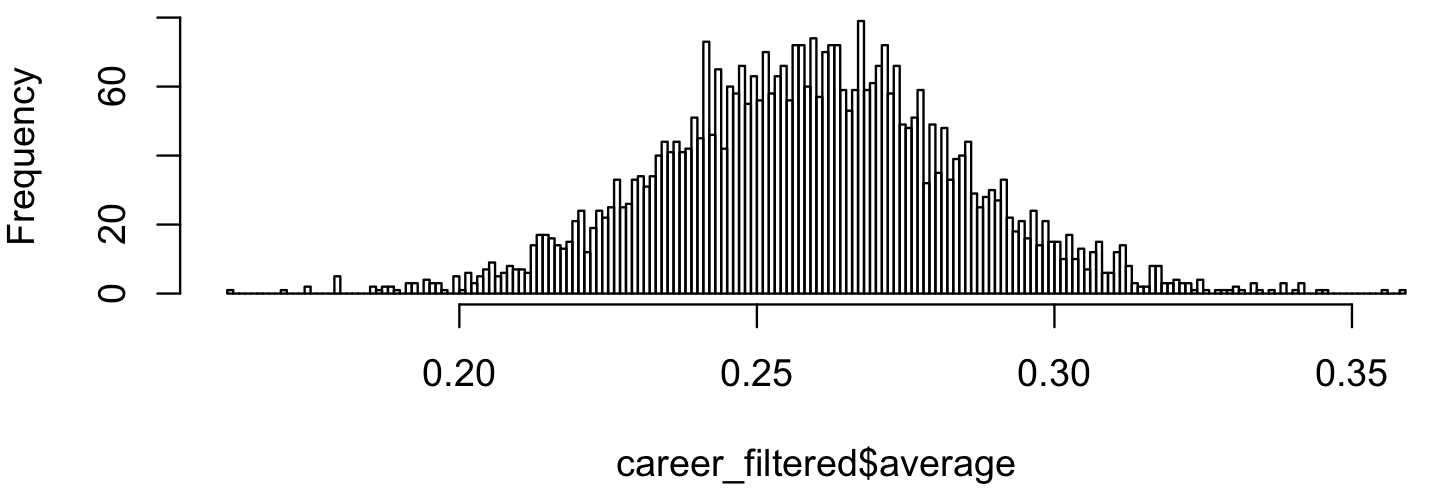
\includegraphics[width=3.5in]{images/bas.png}
\end{figure}

\end{frame}

\begin{frame}[fragile]
	\frametitle{Maximum Likelihood Estimates of $\alpha$ and $\beta$}
	
\scriptsize
We now fit a beta to the historical $\theta$ estimates, plot atop and obtain the MLE's of $\alpha$ and $\beta$:

\begin{verbatim}
m <- MASS::fitdistr(career_filtered$average, dbeta,
                    start = list(shape1 = 1, shape2 = 10))
alpha0 <- m$estimate[1]
beta0 <- m$estimate[2]
round(alpha0, 1) # 79.0
round(beta0, 1) #225.9
hist(rbeta(10000, alpha0, beta0), br = 200, col = "red", prob = TRUE)
hist(career_filtered$average, br = 200, col = "blue", add = TRUE, prob = TRUE)
\end{verbatim}
\vspace{-0.5cm}\pause 

\begin{figure}[htp]
\centering
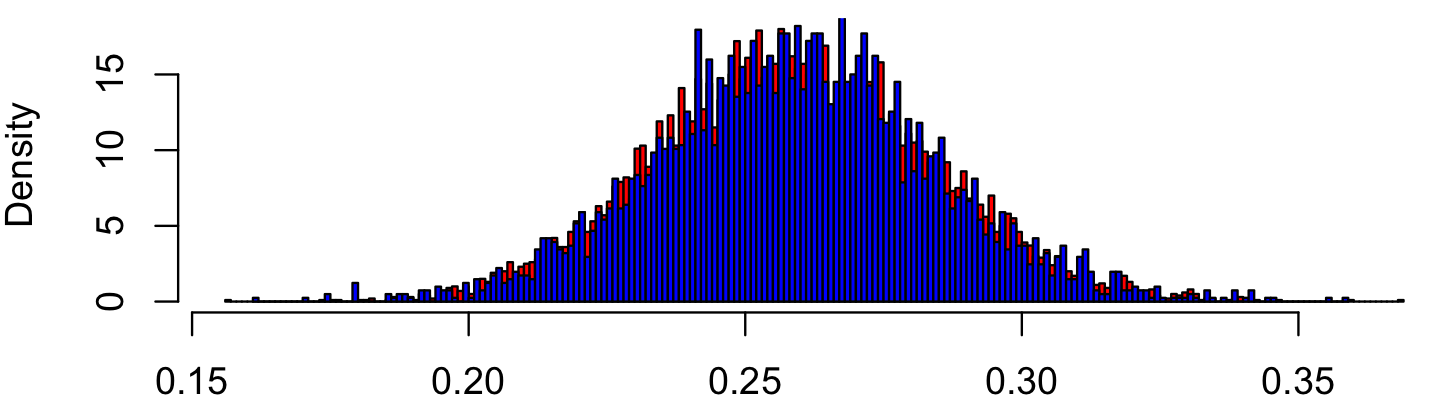
\includegraphics[width=3.5in]{images/basfit.png}
\end{figure}\pause 

As we can see from the agreement of the red (the fit beta) and the blue (the true data), the $\theta \sim \betanot{79.0}{225.9}$ is a very nice fit for the data!
\end{frame}

\begin{frame}
	\frametitle{Empirical Bayes Estimates}

\scriptsize
So now let's use the prior and we get a posterior of:

\beqn
\theta~|~X \sim \betanot{x + 79.0}{n -x + 225.9}
\eeqn\pause 

where the expectation (best Bayesian estimate) is:

\beqn
\cexpe{\theta}{X} = \frac{x + 79.0}{n + 304.9}
\eeqn\pause 

Now we can return to our problem, with two at bats, what are the best estimates?

\beqn
\cexpe{\theta}{X} = \frac{0 + 79.0}{2 + 304.9} = 0.257 \neq 0, \pause ~~ \cexpe{\theta}{X} = \frac{2 + 79.0}{2 + 304.9} = 0.264 \neq 1
\eeqn\pause 

We found that our $0/2$ got shrunk up to 0.257 \pause and our $2/2$ got shrunk down to 0.264. \pause  \qu{Shrinking} means moving towards the prior mean $\alpha / (\alpha+\beta) = 79.0 / 304.9 = 0.259$. \pause This is a \emph{very} good strategy in practice ---\pause  if you don't have any data, \pause pretend this player is like the average player all throughout history!

\end{frame}

\begin{frame}
	\frametitle{Homework Problems}
\begin{enumerate}
\item[1] What is empirical Bayes estimation?
\item[2] Repeat the exercise of building an empirical Bayes estimator with all players who had more than 600 at bats. What are the $\alpha$ and $\beta$ MLE estimates?
\item[3] Verify the beta density with the estimates from (2) is a good fit for the historical data.
\item[4] What is the posterior mean?
\item[5] Use your estimates from (2) to estimate the batting average of a hitter with 5 at bats and 3 hits.
\item[6] What is the probability this hitter from (5) has a BA greater than 300?
\item[7] Provide a credible region for the BA from the hitter of (5).
\item[8] What kind of evidence would be required under (2) for a batter to have a BA estimate of 500?
\end{enumerate}
\end{frame}	

\section{Conclusions}

\begin{frame}
	\frametitle{Outline}

\begin{itemize}
\item Random Variables, the Bernoulli and Binomial simple probability models 
\item Parameters, Estimators and Estimates, Maximum Likelihood 
\item The main problem with the Frequentist Estimator
\item Bayesian Machinery for the binomial likelihood model
\item The Objective / Reference / Uninformative Prior
\item Posterior Distribution, Bayesian Estimate, Credible Intervals
\item Empirical Bayes
\item Estimating Batting Averages with \texttt{R}
\end{itemize}\pause 

You now know how to do all of this!
\end{frame}


\begin{frame}
	\frametitle{Outline for Next Module!}
\pause 
\begin{itemize}
\item Posterior Predictive Distributions, interevals and estimates --- given a Bayesian setup, what will happen in the future? \pause 
\item Bayesian Hypothesis Testing --- how to do tests on $\theta$. \pause 
\item Hierarchical Models --- we know the empirical Bayes models is wrong since BA changes over time and differs by field position of the player (e.g. pitches have lower BA's than outfielders). \pause 
\item Other models besides the beta-binomial model. \pause 
\item Cross-validation for assessing how good the Empirical-Bayes estimates are in practice for real data.
\end{itemize}
\end{frame}

\end{document}
